\documentclass[10pt,oneside,final]{article}
\usepackage[top=1in, bottom=1in, left=1in, right=1in]{geometry}

\usepackage[pagestyles]{titlesec}
\usepackage[margin=10pt,font=small,labelfont=bf, labelsep=endash, justification=centering]{caption}
\usepackage{fancyhdr}
% \usepackage{refcheck}
\usepackage{wrapfig}

\newcommand{\vsp}{\hspace{8pt}}
\newcommand{\vq}{$'$}
\newcommand*\ruleline[1]{\par\noindent\raisebox{.8ex}{\makebox[\linewidth]{\hrulefill\hspace{1ex}\raisebox{-.8ex}{#1}\hspace{1ex}\hrulefill}}}

\titleformat{\chapter}[hang]{\LARGE \sc \filcenter}{\thechapter\vsp}{7pt}{\LARGE \sc}
\titlespacing*{\chapter}{0pt}{0pt}{0pt}

\titleformat{\section}[hang]{\Large \sc \filcenter}{\thesection\vsp}{7pt}{\Large \sc}
\titlespacing*{\section}{0pt}{0pt}{0pt}

\titleformat{\subsection}[hang]{\large \sc  \filcenter\bfseries}{\thesubsection\vsp}{7pt}{\bfseries \large \sc}
\titlespacing*{\subsection}{0pt}{0pt}{0pt}

\titleformat{\subsubsection}[hang]{\normalsize \bfseries \sc \filcenter}{}{0pt}{\bfseries \sc}
\titlespacing*{\subsubsection}{0pt}{0pt}{0pt}

\titleformat{\paragraph}[hang]{\normalsize \sc}{}{0pt}{\sc}
\titlespacing*{\paragraph}{0pt}{0pt}{0pt}

\titleformat{\subparagraph}[hang]{\small \sc}{}{0pt}{\sc}
\titlespacing*{\subparagraph}{0pt}{0pt}{0pt}

% \newcommand{\vsp}{\hspace{8pt}}
% \titleformat{\section}[hang]{\Large \sc \filcenter}{\thesection\vsp}{7pt}{\Large \sc}
% \titlespacing*{\section}{0pt}{0pt}{0pt}
% \titleformat{\paragraph}[hang]{\normalsize \sc \filcenter}{}{0pt}{\sc}
% \titlespacing*{\paragraph}{0pt}{0pt}{0pt}
\usepackage{amsmath,amssymb,amstext}
\usepackage[pdftex]{graphicx}
\usepackage[pdftex,pagebackref=false]{hyperref} % with basic options
        % N.B. pagebackref=true provides links back from the References to the body text. This can cause trouble for printing.
\hypersetup{
    plainpages=false,       % needed if Roman numbers in frontpages
    pdfpagelabels=true,     % adds page number as label in Acrobat's page count
    bookmarks=true,         % show bookmarks bar?
    unicode=false,          % non-Latin characters in Acrobat’s bookmarks
    pdftoolbar=true,        % show Acrobat’s toolbar?
    pdfmenubar=true,        % show Acrobat’s menu?
    pdffitwindow=false,     % window fit to page when opened
    pdfstartview={FitH},    % fits the width of the page to the window
    pdftitle={SYDE 552 - Assignment 3},    % title: CHANGE THIS TEXT!
    pdfauthor={Prajna Kandarpa},    % author: CHANGE THIS TEXT! and uncomment this line
    pdfsubject={},  % subject: CHANGE THIS TEXT! and uncomment this line
    pdfkeywords={brain} {neuroscience} {ventral} {intraparietal}, % list of keywords, and uncomment this line if desired
    pdfnewwindow=true,      % links in new window
    colorlinks=true,        % false: boxed links; true: colored links
    linkcolor=blue,         % color of internal links
    citecolor=magenta,        % color of links to bibliography
    filecolor=magenta,      % color of file links
    urlcolor=cyan           % color of external links
}
% \hypersetup{  % override some previously defined hyperref options
% %    colorlinks,%
%     citecolor=black,%
%     filecolor=black,%
%     linkcolor=black,%
%     urlcolor=black}
% \usepackage[pdftex,letterpaper=true,pagebackref=false]{hyperref}
% \linespread{value}
% where value determine line spacing. This value is somewhat confusing, because:
% Value Line spacing
% 1.0   single spacing
% 1.3   one-and-a-half spacing
% 1.6   double spacing
\linespread{1.3}
\title{Visual Cortex Literature Review}
\author{Prajna Kandarpa - 20402024}
\begin{document}
    % \pagestyle{empty}
    \pagenumbering{arabic}
    \maketitle
    \section{Introduction} 
        % \paragraph{Prajna Kandarpa - \#20402024}
        % \vspace{0.4cm}
        % \subsection*{Introduction}
        \begin{wrapfigure}{r}{0.5\textwidth}
            \centering
            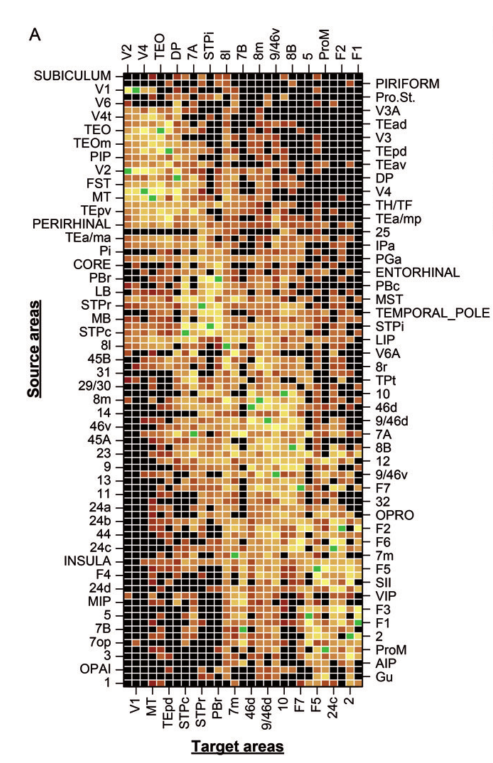
\includegraphics[width=0.5\textwidth]{area_heatmap}
            \caption{Connectivity Matrix represented as a heatmap for a macaque brain \cite{Markov2014}}
            \label{fig:heat}
        \end{wrapfigure}
        One of the primary tasks of the human brain is to generate rich representations of space including objects and organisms using their sensory epithelia\cite{Duhamel1998}. The parietal lobe is one of the four major lobes of mammal brains and is positioned above the occipital lobe and behind the frontal lobe and central sulcus. The intraparietal sulcus is located on the lateral region of the parietal neocortex and consists of about 5 functionally distinct subregions that have been intensively investigated using both single cell neurophysiology in primates and human functional neuroimaging. - anterior, lateral, ventral, caudal, and medial corresponding to the names AIP, LIP, VIP, CIP and MIP. Its principal functions are related to perceptual-motor coordination and auxiliary functions are related to processing symbolic numerical information and visuospatial working memory. 

        According to \cite{Duhamel1998}, the posterior parietal cortex contains several distinct regions that are part of the dorsal stream visual pathway.This literature review will focus on the Ventricular Intra-Parietal (VIP) area of the macaque brain, which primarily receives input from the visual, somato-sensory, auditory and vestibular systems, with one of its major sources of input being the medial temportal area (MT). The VIP area is used in perceiving touch, extra near personal space and optic flow\cite{kruger2013deep}.
        % \clearpage
        Figure \ref{fig:heat} shows an interconnectivity matrix between the different regions of the macaque brain. From this matrix, the row corresponding to the VIP target area, shows high number of connections to the regions labeled 5, 9/46d, 8m, 7B, 7m, 8l, MT and DP regions. The lateral locations of these regions on a flat map in the macaque brain are as follows:
        \begin{enumerate}
            \item{Area 5 - Located next to the MIP and is part of the parietal cortex}
            \item{Areas 9/46d- Located in the prefrontal cortex}
            \item{Area 8m - Located in the prefrontal cortex}
            \item{Area 8l - Located in the prefrontal cortex}
            \item{Area 7B - Located in the parietal cortex}
            \item{Area 7m - Located in the parietal cortex}
            \item{Area MT - Stands for the medial temporal, located in the superior temporal sulcus}
            \item{Area DP - Stands for Dorsal Prelunate Area. Corresponds very closely to V4 in the brain.}
        \end{enumerate}

        This review intends to analyze the results of 3 different papers that explore the properties of the VIP area in the macaque. Important topics of interest include cell selectivity for directions of multiple sensory modalities, corresponding cell spike rates and response latencies.

    \section{Duhamel et al 1998}
        The authors of this paper \cite{Duhamel1998}, used two types of separate blocks of trials - visual and somatosensory with appropriate rewards for the completion of both tasks. Aim of the study was to prove that an area previously thought to contain only one kind of VIP neurons actually contained both visual and somatosensory neurons. They were able to estimate amplitudes of the neuronal responses but not latencies. 218 neurons in the VIP area were independently tested and their responses to both kinds of stimuli was measured. 153 cells responded to both sensory modalities while 70 responded only to visual stimuli. None of the neurons responded only to tactile stimulation.
        \begin{figure}[h!]
            \centering
            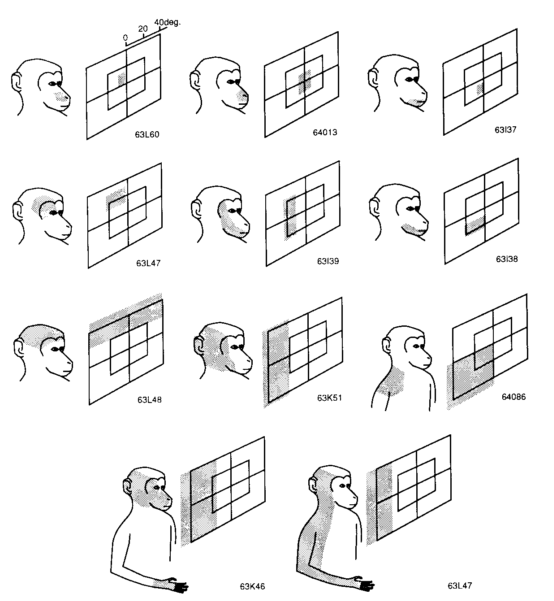
\includegraphics[width=0.5\textwidth]{duhamel_bimodal_rf.png}
            \caption{Visual and somatosensory receptive fields for 11 different VIP neurons. Each axis represents angles from the center of reference in the corresponding axis' directions\cite{Duhamel1998}}
            \label{fig:duh_rf}
        \end{figure}
        In Figure \ref{fig:duh_rf}, location and contours of visual and tactile receptive fields (RFs) are shown for 11 different neurons. The tactile RFs shown in the top row vary in size from small ($1-8 cm^2$) to quite large (body sized). Most RF's were found on the contralateral side of the body (72\%), 10\% were found on the ipsilateral side and 18\% on the midsagittal line.
        \begin{figure}[h!]
            \centering
            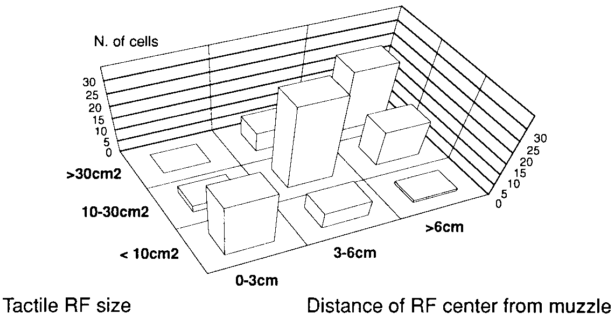
\includegraphics[width=0.5\textwidth]{duhamel_RF_sizes.png}
            \caption{Relation between tactile RF size and location for population of bimodal VIP neurons \cite{Duhamel1998}}
            \label{fig:duf_rf_sizes}
        \end{figure}
        Figure \ref{fig:duf_rf_sizes} shows that small RF's were located very close to the lips and nose, while larger RF sizes were found on top, side or back of the head and the neck. It also shows the size of the RF increased as the RF's radial distance from the muzzle increased. Drawing an analogy to the visual system, the face may be thought of as a somatosensory \textit{fovea} for the VIP area. 

        Visual activity in the VIP area is characterized by its selectivity for speed and direction of visual stimuli in the frontoparallel plane. Selectivity was seen in the neurons for direction of movement for the tactile and visual stimuli involving a small object. A specific neuron presented in the paper responded selectively to a leftward moving stimulus for both sensory modalities. The poststimulus time histogram showed a peak frequency of 200 impulses/s for the leftward moving stimuli for a spot of light moving at a speed of 40 [deg/s] across the RF. Another neuron studied was subject to a different kind of stimulus, this time a large object moved front to back and reverse in the far contralateral visual periphery while the monkey fixated on the tangent screen. This time, the neuron exhibited selectivity for stimuli going towards the face in both visual and somatosensory modalities. The peak rates in the PSTH were slightly more than 200 impulses/s for this kind of input in the neuron's preferred direction. The histogram also exhibited greater distribution of higher impulse rate bins than the earlier case of a smaller stimuli closer to the face. Most bimodal neurons exhibited congruent direction selectivity for both sensory modalities. 

        Parallel visual and tactile motion direction selectivity was recorded in cells with both peripheral and central RFs. VIP neurons that respond best to stationary or moving 3-d objects in close interpersonal space did not respond at all to visual stimuli on the tangent screen. No topographic grouping was found to imply a retinotopic or somatotopic organized map in the distribution of bimodal and visual only VIP neurons. The most frequent response pattern in VIP is characterized by congruent preferred directions for moving visual and tactile stimuli. VIP may be unique in containing a majority of such bimodal direction selective neurons.
    \section{Duhamel et al 1997}
        The aim of this study was to differentiate between neurons in the VIP area with RF's whose reference frames are either centered on the eyes or centered on the head. They showed that the activity of visual neurons in VIP is modulated by eye-position signals, as in many other areas of the cortical visual system. We find that individual receptive fields of a population of VIP neurons are organized along a continuum, from eye to head coordinates. In the latter case, neurons encode the azimuth and/or elevation of a visual stimulus, independently of the direction in which the eyes are looking, thus representing spatial locations explicitly in at least a head-centred frame of reference\cite{Duhamel1997}.

        The RFs of the neurons studied are plotted in two different coordinate systems - head centered and eye centered to help identify selectivity towards either or a hybrid reference frame. Some neurons had RF's that moved rigidly with eyes with displacements dependent on the eye displacement although its not necessarily a linear relationship. 
        \begin{figure}[h!]
            \centering
            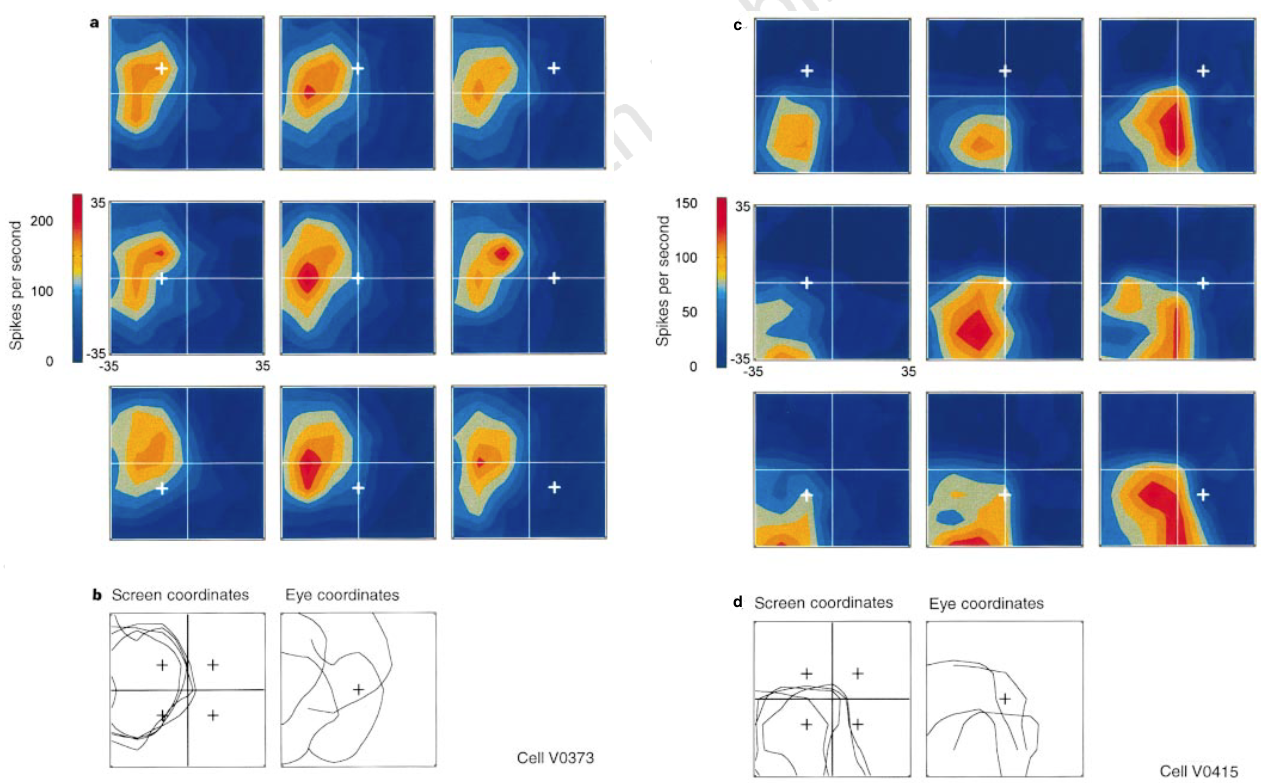
\includegraphics[width=\textwidth]{duh_contour.png}
            \caption{\textbf{a.} Contour heatmap of spike rates overlaid on screen coordinates for an eye position independent neuron. \textbf{b.} Each outline shows the screen region where the spike rates were greater than 50\% of mean rates. \textbf{c.} Contour heat map for a neuron encoding elevation changes. \textbf{d.} Each outline shows the screen region where the spike rates were greater than 50\% of mean rates. \cite{Duhamel1997}}
            \label{fig:duh_cont}
        \end{figure}

        Fig. \ref{fig:duh_cont} shows the neural activity distribution over the simulated screen area for 9 different eye fixation locations for two types of neurons, eye location independent and dependent. Fig. \ref{fig:duh_cont}a shows a neuron that fixates on the same spatial point regardless of eye direction. This indicates that it does not encode a fixed retinal location but the retinal location changes with movement of the eye so as to drive the neuron with information for a specific location in space. These neurons exhibit complete compensation for eye displacements. 

        Fig. \ref{fig:duh_cont}b shows a neuron whose RF remained fixed on the same point on the screen for vertical eye movements but changed slightly for horizontal eye movements is presented. To quantify the extent to which an RF moves with the eyes, the authors applied two-dimensional cross-correlation between the nine different maps obtained for the same cell. This helps define how much an RF map obtained at a given fixation must be shifted relative to a map obtained at a different position in order to maximize the correlation coefficient. For head-centred RFs, the highest correlation is obtained when the two maps are perfectly superimposed (null shift), whereas for eye-centred RFs, it is obtained when the maps are shifted by an amount equal to the difference in eye position between the two mapping conditions. Thus, the expected ratio of the computed shift to the difference in eye position is 0.00 for head-centred RFs, and 1.00 for eye-centred RFs. 

        It seems that although RF shifts as a function of eye position are measured on a continuous scale, the population of VIP neurons studied might actually contain two distinct subpopulations of RF types, linked by an area of gradual transition between retinal and head-centred coordinates. The authors of this paper did not focus too much on the spike rates or response latency.
    \section{Avillac et al 2007}
        The goal of this study was to characterize multisensory interaction patterns in the cortical ventral intraparietal area (VIP) of the macaque. They found that \textgreater70\% of the 150 neurons studied in this experiment integrated visual and tactile events. The multisensory integration took place on the discharge rates and response latency of both multimodal and unimodal neurons. 

        The authors used two slightly modified multisensory indices to measure neuronal spike discharge rates and latency with statistical confidence. The first one reflects the enhancive or suppressive effects of adding a second stimulus modality and compares the bimodal response of the neuron with the maximal unimodal response. \cite{meredith1983interactions}. The second one was a multisensory contrast index, directly evaluates the super-additivity hypothesis by comparing the bimodal response with the sum of the two unimodal responses (V for visual, T for tactile) \cite{laurienti2005use}. 
        
        They recorded single-unit activity in two alert monkeys during the presentation of visual (drifting gratings) and tactile (low-pressure air puffs) stimuli. 150 cells in VIP in two behaving monkeys (96 in monkey N and 54 in monkey M) were recorded. Most of the recorded neurons were bimodal visual–tactile (87 of 150, 58\%), 35\% were exclusively visual (53 of 150), and a minority was exclusively tactile (10 of 150, 7\%) (t test, p < 0.05 corrected).More than 70\% of VIP cells showed a significant modulation of their response by bimodal stimulations. These cells included both bimodal cells, i.e., cells responsive to both tested modalities, and seemingly unimodal cells, i.e., cells responding to only one of the two tested modalities. 

        A neuron is classically defined as unimodal when it responds to one sensory modality and is totally insensitive to the presentation of stimuli from other sensory modalities. The authors found that a stimulus that is ineffective at eliciting a response (mean firing rates) from the neuron when applied on its own would affect the neuron's response when combined with stimuli of other sensory modalities. This seems to indicate that even the seemingly unimodal neurons were actually integrating multiple sensory modalities in VIP. 

        For bimodal neurons, the peak rate in PSHT for a tactile input was around 50impulses/s, 80impulses/s for visual input and 100impulses/s for bimodal input(Values presented for a single cell) for an enhancing multisensory integration. The corresponding values for depressive multisensory integration were 150impulses/s, 45impulses/s and 100impulses/s. For unimodal neurons, the peak PSHT rate was 45 impulses/s for tactile input, ~10impulses/s for visual input and 100impulses/s for bimodal inputs for enhancing multisensory integration. for depressive multisensory integration in unimodal neurons, the corresponding rates were 25impulses/s for tactile, 200impulses/s for visual and 150impulses/s for bimodal inputs. These figures prove the enhancing and depressive effects of multisensory integration for both bimodal and unimodal neurons.

        In essence, the authors found two kinds of multisensory integrative cells in the VIP area. 
        \begin{itemize}
            \item{The first kind would respond to one sensory modality and not respond at all to other modalities. However, these neurons would change their response when the stimuli they don't respond to individually were integrated with stimuli of modalities they are sensitive to. The change in response was either enhancing(33\%) or depressive(67\%) compared to the unimodal case. }

            \item{The second kind of neurons responded equally well to both visual and tactile stimuli individually and also responded to multi modal stimuli with an enhanced or depressive response compared to the unimodal stimulus case.}
        \end{itemize}
        \begin{figure}[h!]
                \centering
                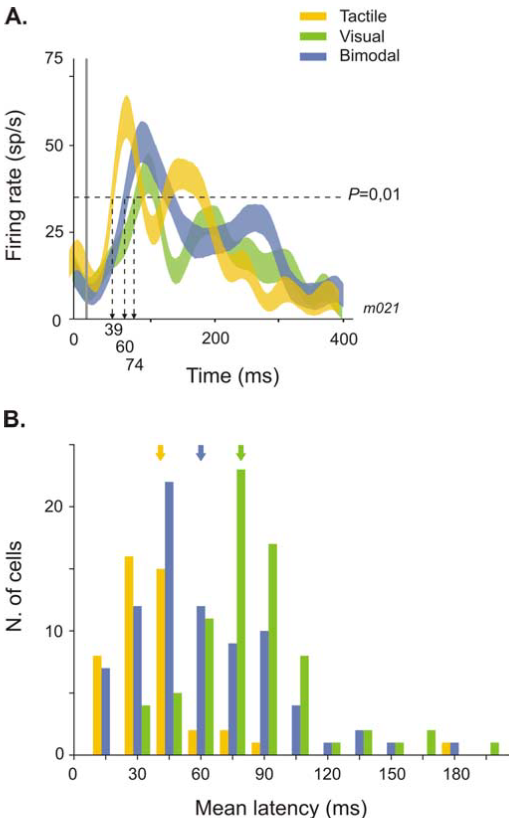
\includegraphics[width=0.5\textwidth]{schlack_latency.png}
                \caption{Multisensory integration effects on neuronal latency \textbf{A.}Single cell results. \textbf{B.}Latency distribution for VIP neuron population\cite{Avillac2007}}
                \label{fig:sch_lat}
        \end{figure}
        Fig. \ref{fig:sch_lat} shows the distribution of bimodal, tactile and visual latencies for the studied population of neurons. Tactile latencies($41.5 \pm 3.5$ms) were found to be significantly lower than visual latencies($85 \pm 3$ms). No significant differences were found between integrative and non integrative neuron latencies to unimodal stimuli. Response latency to bimodal stimuli was $68.8 \pm 3.1$ms, which is significantly shorter than unimodal visual latency but significantly greater than unimodal tactile latency. A marginally significant difference in bimodal response latency was found between integrative and non-integrative cells suggesting that the multisensory effects on latencies could be dependent on discharge rate \cite{Avillac2007}.

        Thus, the authors showed that the majority of VIP neurons integrate multisensory stimuli. Even though they only covered visual and tactile stimuli, its quite possible that these results can also be reproduced for other forms of sensory modalities that VIP is sensitive to, such as auditory inputs \cite{Schlack2005}.
    \section{Conclusion}
        The three papers reviewed in this report give a sense of the various functions hypothesized to be performed by the ventral intraparietal area. It is important to note that the VIP area has confounded and confused people a lot because of the ambiguous nature of its role in the dorsal stream. The fact that it's activated as part of the dorsal pathway seems to hint at its importance for visual analysis.

        Some VIP neurons have tactile (touch) receptive fields that can represent space in a head centered reference frame. Other types of VIP neurons are thought to have visual receptive fields and fire with a head centered reference with eye-centered coordinates. VIP neurons exhibited a high degree of selectivity for the direction of a moving stimulus, speed of stimulus motion, distance at which stimulus appears and to/fro movement of stimulus towards the subject. They weren't very active in relation to saccadic eye movements but were slightly more sensitive during smooth pursuit of dynamic stimuli.

        The predominance of neurons selective for direction and speed in area VIP suggests that this area contributes to the analysis of visual motion. It is of particular interest that some VIP neurons appear to be involved in detection of the trajectory of stimulus motion and anticipation of point of contact for an approaching visual stimulus. For most of these neurons, the visual response was tied to the location of the somatosensory receptive field, although some purely visual neurons were also selective for stimulus trajectory \cite{Colby1993}.       



\clearpage
% \nocite{*}
\bibliographystyle{IEEEtran}
% \renewcommand*{\bibname}{References}
\bibliography{20402024_litreview_syde552}
\end{document}


